% LaTeX file for Chapter 02









\chapter{Methodology} 

\section{Definitions}

The \textbf{Target Population} is a specific group within the broader population, defined by attributes relevant to the research question. This group is focused on criteria that match the study's goals \citep{willie2024population}. Defining the target population allows researchers to refine their objectives and recruitment methods to align with the study's aims.


The \textbf{Eligibility} criteria are the specific requirements that individuals must meet to participate in a study. Eligible patients will be selected from the target population. Inclusion criteria specify the conditions that allow individuals to participate in the trial, particularly focusing on the medical condition of interest. Any other factors that limit eligibility are classified as exclusion criteria \citep{van2007eligibility}, conditions or circumstances that disqualify potential participants \citep{food2018evaluating}.


In clinical trials, \textbf{Enrollment} refers to the formal process of registering participants into a study after they have met all eligibility criteria and provided informed consent. This process includes verifying that each participant satisfies the inclusion and exclusion criteria outlined in the study protocol \citep{NIH2021}. It is important to distinguish between recruitment and enrollment. Recruitment involves identifying and inviting potential participants to join the study, whereas enrollment occurs after these individuals have been screened, consented, and officially registered into the trial \citep{frank2004current}. 

Once enrolled, participants are assigned to specific treatment groups or interventions as defined by the study design. The most common practice is \textbf{Randomization}. In clinical research, randomization is the process of assigning participants to different treatment groups using chance methods, such as random number generators or coin flips \citep{lim2019randomization}. Randomized controlled trials (RCTs) are considered the most effective method for preventing bias in the evaluation of new interventions, drugs, or devices. \citep{van2007eligibility}.


In clinical research, \textbf{Statistical Analysis} involves applying statistical methods to collect, summarize, interpret, and present data derived from clinical studies. This process is essential for evaluating the safety, efficacy, and overall outcomes of medical interventions, ensuring that conclusions drawn are both reliable and valid \citep{panos2023statistical}. Not all participants who are randomized may be included in the final statistical analysis due to protocol deviations of patients not adhering to the protocol \citep{rehman2020exclusion}, missing data \citep{shih2002problems} or loss-to-follow-up, some participants may become unreachable or withdraw consent during the study, resulting in missing outcome data \citep{nuesch2009effects}.

\begin{figure}[h]
  \centering
  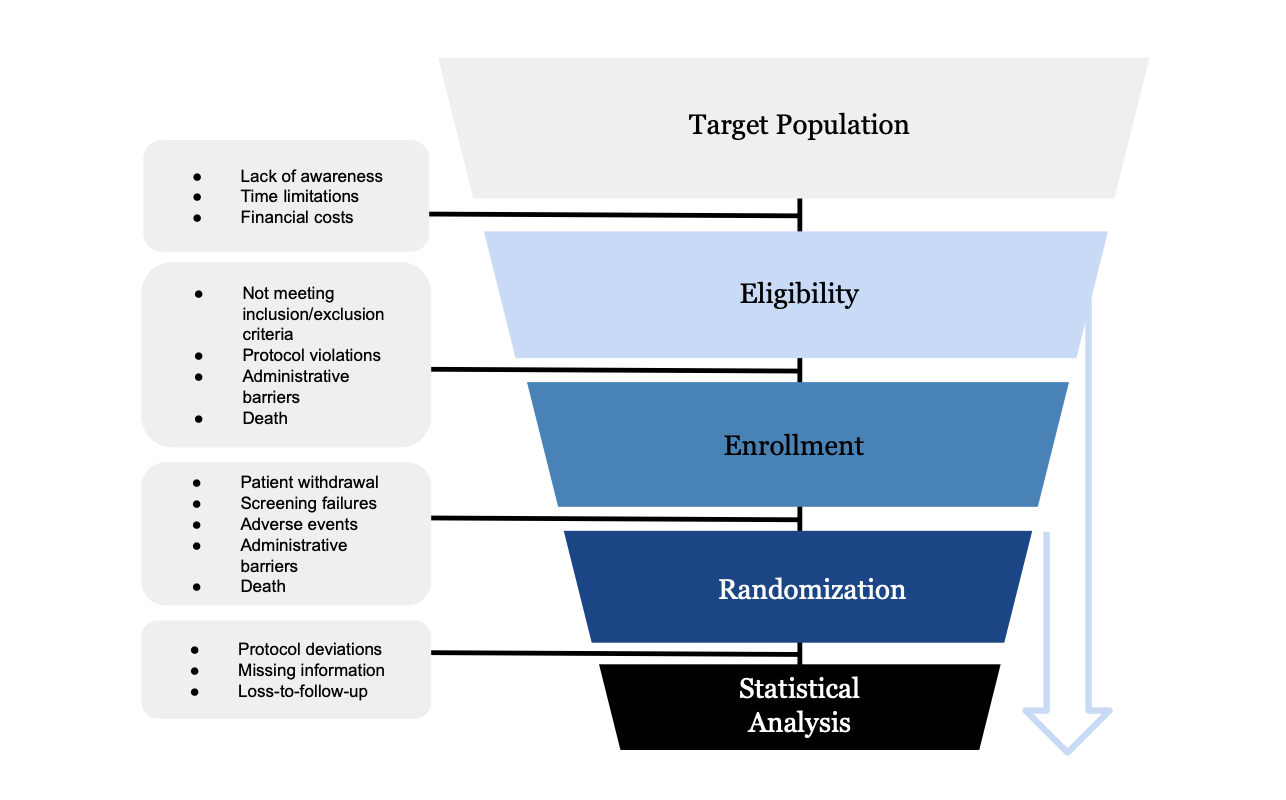
\includegraphics[width=0.7\textwidth]{fig_2_1_a.png}
  \caption{Patient Attrition at Each Stage of a Clinical Study.  \citep{piantadosi2022principles, whelan2018high, bogin2022lasagna}}
  \label{fig:2_1_a}
\end{figure}

The number of patients decreases at each stage of a clinical study, from defining the target population to final statistical analysis, see Figure \ref{fig:2_1_b}. Eligibility criteria narrow down participants, and enrollment further reduces numbers as only those meeting strict criteria are registered. Randomization assigns individuals to treatment groups, but some may later be excluded due to protocol deviations, missing data, or loss to follow-up. 

The general notion of \textbf{Recruitment} in this Master Thesis refers to the number of patients (Counts) at the Eligibility, or Enrollment, or Randomization, or Statistical Analysis stage in Figure \ref{fig:2_1_a}. We define \textbf{Accrual} as cumulative recruitment.

\begin{figure}[h]
  \centering
  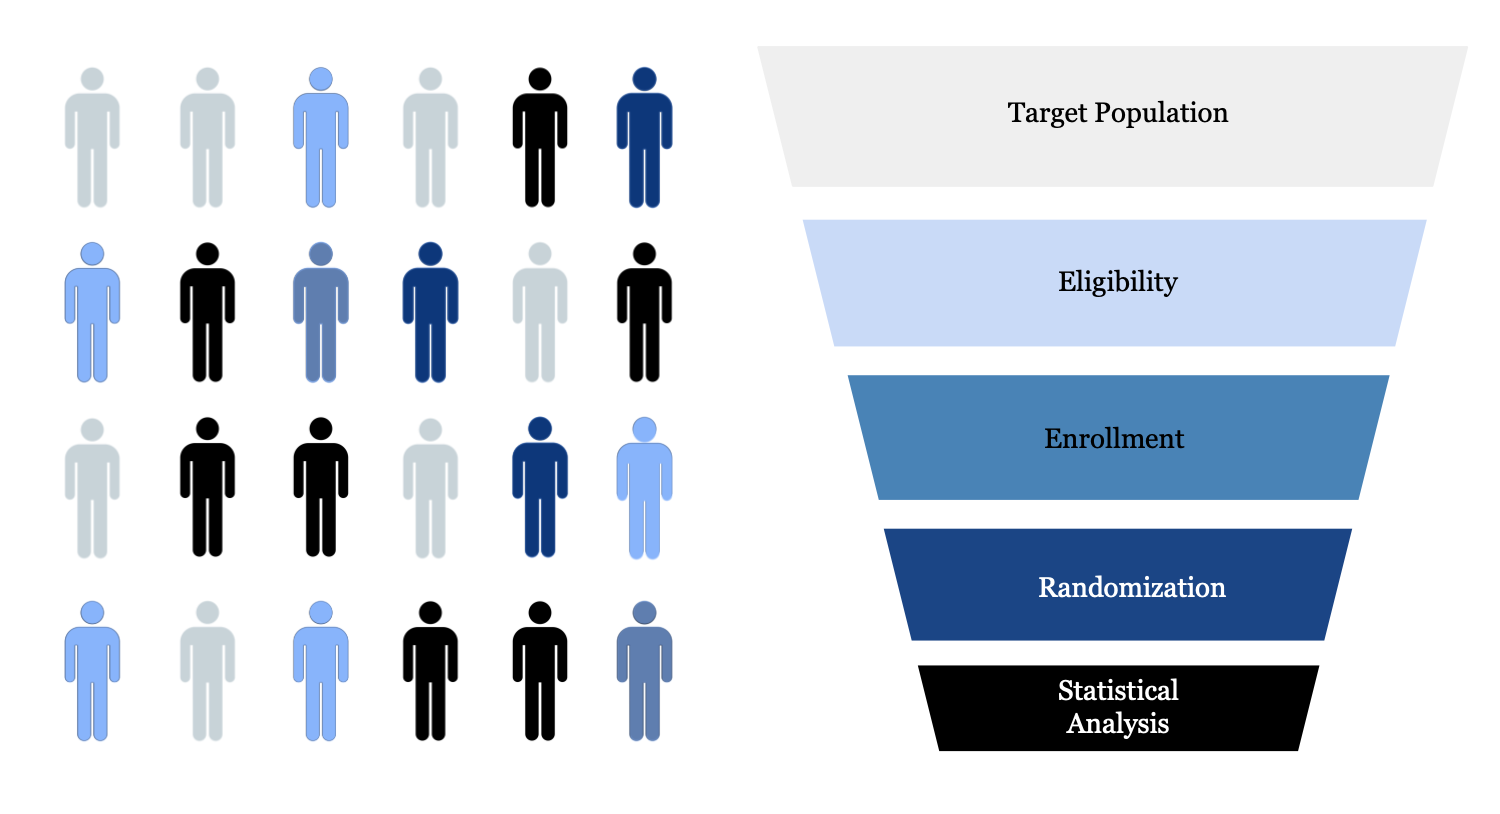
\includegraphics[width=0.7\textwidth]{fig_2_1_b.png}
  \caption{Visual Representation of Patient Leakage at Each Stage of a Clinical Study.  \citep{piantadosi2022principles, whelan2018high, bogin2022lasagna}}
  \label{fig:2_1_b}
\end{figure}

\section{Uncertainty and models for counts}

There are two types of uncertainty, aleatory and epistemic \citep{ohagan2006}. The \textbf{Aleatory Uncertainty} reflects randomness that is inherent, irreducible and unpredictable in nature. \textbf{Epistemic Uncertainty} arises primarily from limited or imperfect knowledge about the parameters of a statistical model. Obtaining more or better information about the parameter reduces the epistemic uncertainty. 

Let us denote

\begin{itemize}
\item $T=time$
\item $C=counts$
\item $\lambda=\frac{C}{T}$
\end{itemize}

\begin{table}[h!]
\centering
\resizebox{\textwidth}{!}{
\begin{tabular}{cccccc}
 \textbf{Methods} & \textbf{Counts} & \textbf{Expectation} & \textbf{Variance} & \textbf{Aleatory} & \textbf{Epistemic} \\
\hline
\hline
Expectation & $C = \lambda  t$ & $\lambda  t$ & 0 & No & No \\
Poisson & $C \sim \rm{Po} (\lambda  t)$ & $\lambda  t$ & $\lambda  t$ & Yes & No \\
Negative Binomial & $C \sim \rm{Po} (\Lambda  t)$; $\Lambda \sim \rm{G}(\alpha,\beta)$ & $\frac{\alpha}{\beta}$ & $\frac{\alpha(\beta+1)}{\beta^2}$ & Yes & Yes \\
\end{tabular}
}
\caption{Aleatory and epistemic uncertainty in accrual shown by different models for counts.}
\label{tab:count_modeling}
\end{table}

\section{Counts: Model based on Expectations}

If we fix a time $T$ for the study to take place and we must enroll $N$ patients, we could deterministically predict our recruitment rate (without taking into consideration any uncertainty) to be $\hat{\lambda}=\frac{N}{T}$ . 

However, by normal approximation to the Poisson distribution $T\sim \rm{N}(\mu=N, \sigma^2=N)$, we know that the probability of recruiting the desired $N$ participants is 0.5. Which means that the study has 50\% chance of obtaining the desired sample size in the suggested $T$ \citep{carter2004application}. We would also be assuming that the recruitment rate is constant over time.

This raises two questions which will be answered throughout this Master Thesis:
\begin{enumerate}
\item \textbf{Counts?:} If $T$ is fixed, what does the expected rate need to be to give a certain percentage of certainty of enrolling the total sample size $N$ within said time frame?
\item \textbf{Time:} Given a certain rate $\lambda$, how long should the recruitment period be planned to give a certain level of confidence of recruiting the total sample size?
\end{enumerate}

\subsection{Expected in one unit of time}
$C = EC = E\lambda = \lambda$

\subsection{Expected accrual at time point t}
$C = EC = E(\lambda t) = \lambda t$

\section{Counts: Model based on Poisson Process}

The Poisson distribution $C\sim \rm{Po} (\lambda)$ allows us to explain the recruitment of patients. It is a discrete variable that expresses the probability of a given number of events (in our case, patient recruitment) occurring in a fixed interval of time. We assume that these events occur with a known constant rate and are independent of each other.

\begin{align*}
EC & = \lambda\\
Var(C) & = \lambda
\end{align*}

One important property from the Poisson distribution is that it is additive \citep{held2014applied}. If $X_i\sim \rm{Po} (\lambda_i)$ for $i=1\cdots n$ are independent, then, $\sum_{i=1}^n X_i \sim \rm{Po} \Big( \sum_{i=1}^n \lambda_i \Big)$.

\subsection{Recruitment in one unit of time}
$C\sim \rm{Po} (\lambda)$

\subsection{Accrual at time point t}
Using the additive property from the Poisson applicable to independent random variables, $\underbrace{\rm{Po} (\lambda) +\cdots +\rm{Po} (\lambda)}_{t \ \text{times}} = \rm{Po} (\lambda t)$, we have that:\\

$C\sim \rm{Po} (\lambda t)$

We assume that the recruitment of patients at a given time point is independent from another.

Here I could reference the figures, since they are all from this section.

\begin{figure}
\begin{knitrout}
\definecolor{shadecolor}{rgb}{0.98, 0.98, 0.98}\color{fgcolor}

{\centering 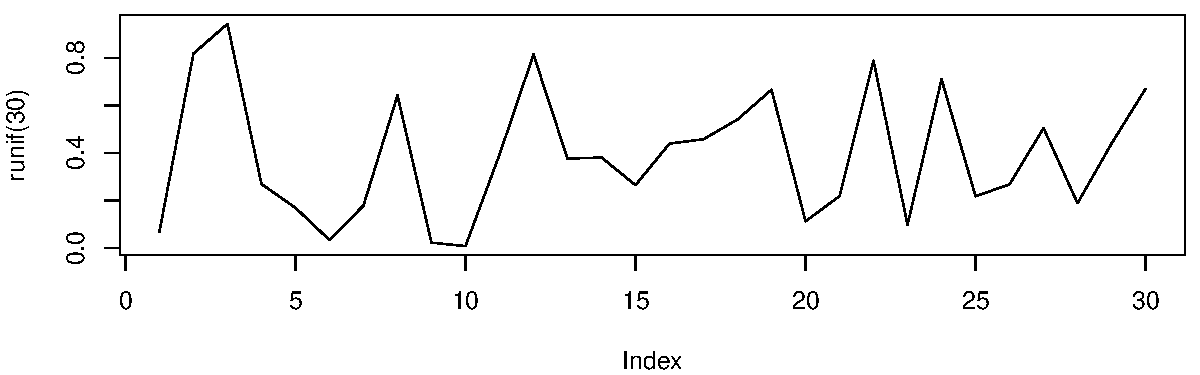
\includegraphics[width=\textwidth-3cm]{figure/ch02_figunnamed-chunk-3-1} 

}


\end{knitrout}
  \caption{Poisson-distributed counts with $\lambda = 0.591$ over time and uncertainty range. The black line represents the point estimate of the expected accrual, while the red dashed lines indicate Poisson's 95\% aleatory uncertainty. The histogram illustrates the distribution of observed counts at time $T = 550$ \citep{spiegelhalter2011visualizing, pkgacc}.}
  \label{fig:2_2}
\end{figure}


\begin{figure}
\begin{knitrout}
\definecolor{shadecolor}{rgb}{0.98, 0.98, 0.98}\color{fgcolor}

{\centering 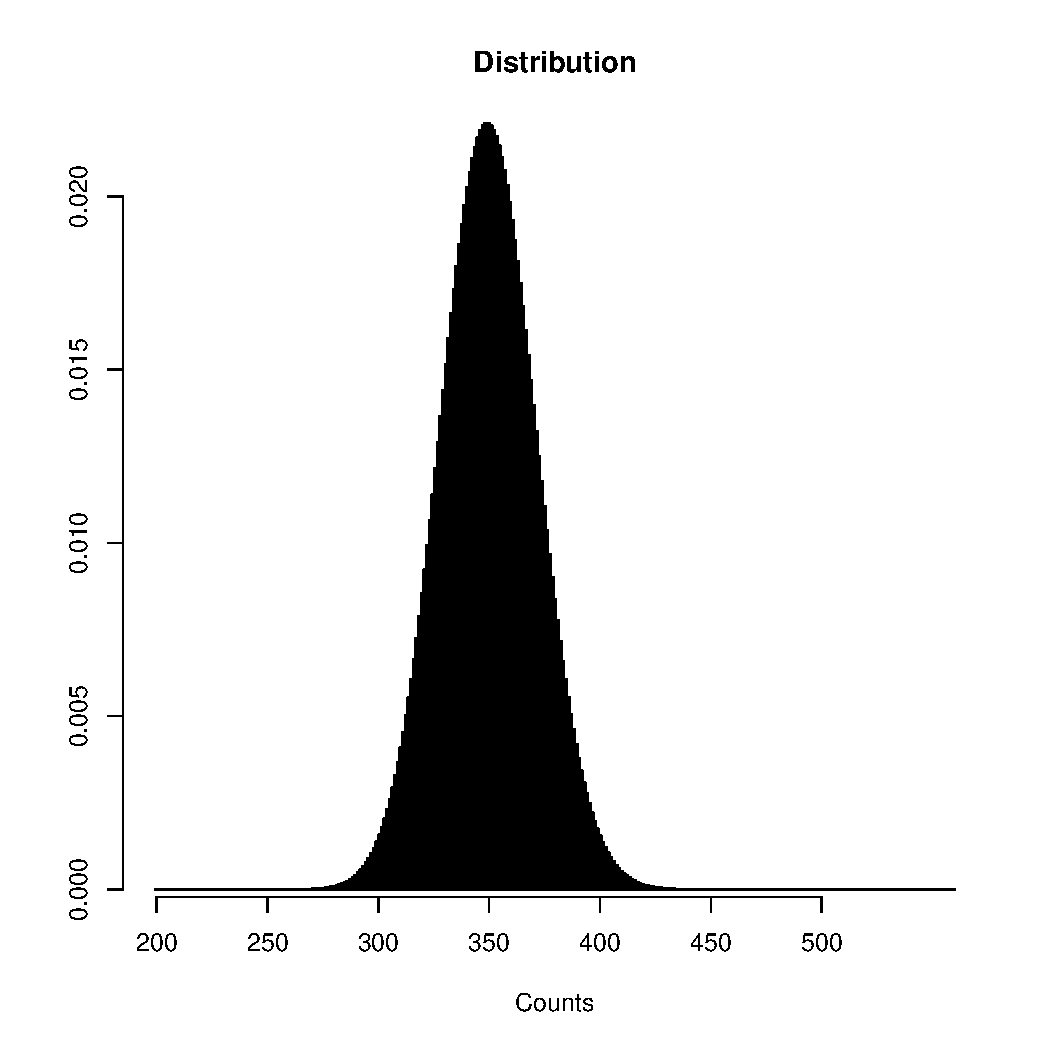
\includegraphics[width=\textwidth-3cm]{figure/ch02_figunnamed-chunk-4-1} 

}


\end{knitrout}
  \caption{Poisson Distribution of Counts: This bar plot represents the probability mass function (PMF) of counts ranging from 200 to 500, using a Poisson distribution with a rate parameter $\lambda = 0.591$ based on 550 time periods.}
  \label{fig:2_3}
\end{figure}

\begin{figure}
\begin{knitrout}
\definecolor{shadecolor}{rgb}{0.98, 0.98, 0.98}\color{fgcolor}

{\centering 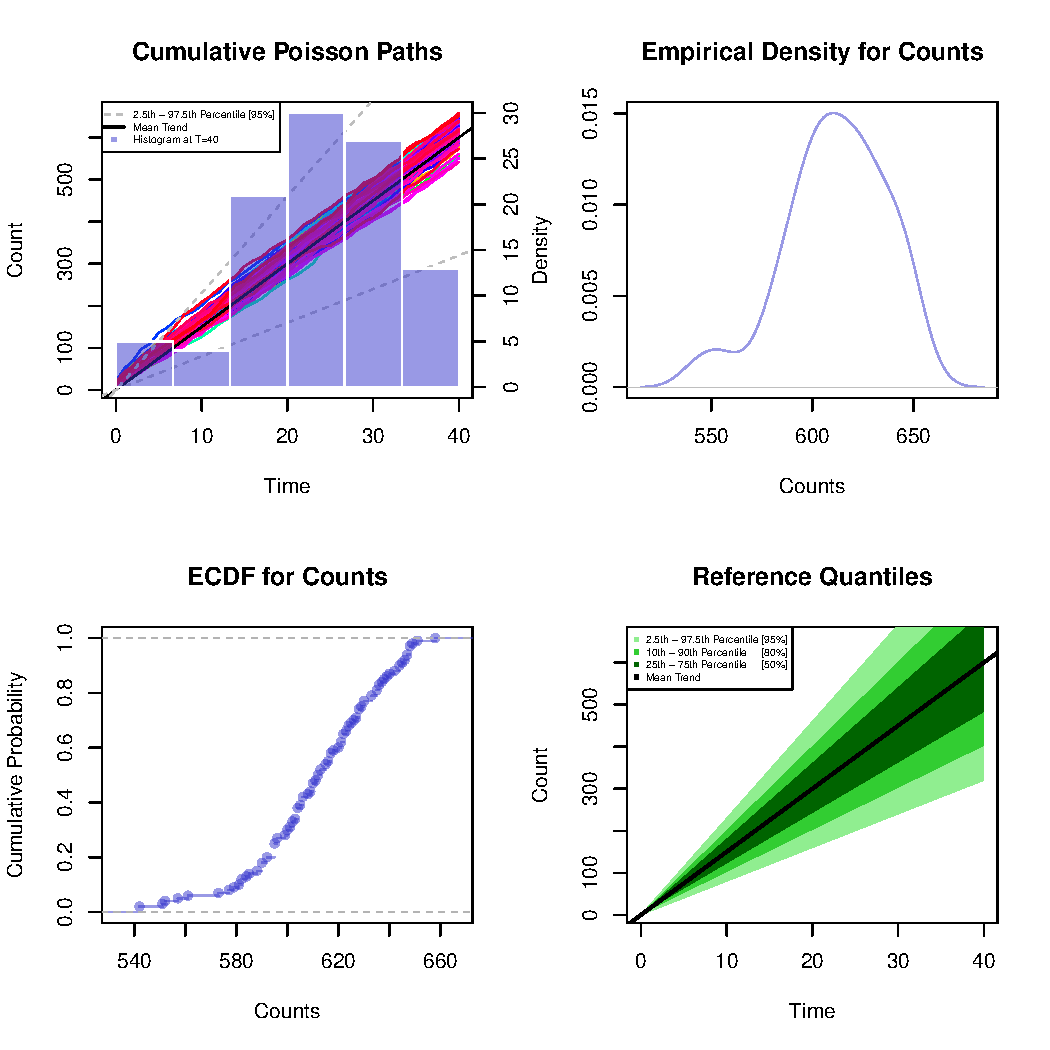
\includegraphics[width=\textwidth-3cm]{figure/ch02_figunnamed-chunk-5-1} 

}


\end{knitrout}
  \caption{Cumulative Distribution of Poisson-Distributed Counts: The plot illustrates the cumulative probability distribution for counts within the range of 200 to 500, using a Poisson distribution with a rate parameter $\lambda = 0.591$ adjusted for 550 time periods.}
  \label{fig:2_4}
\end{figure}


\begin{figure}
\begin{knitrout}
\definecolor{shadecolor}{rgb}{0.98, 0.98, 0.98}\color{fgcolor}

{\centering 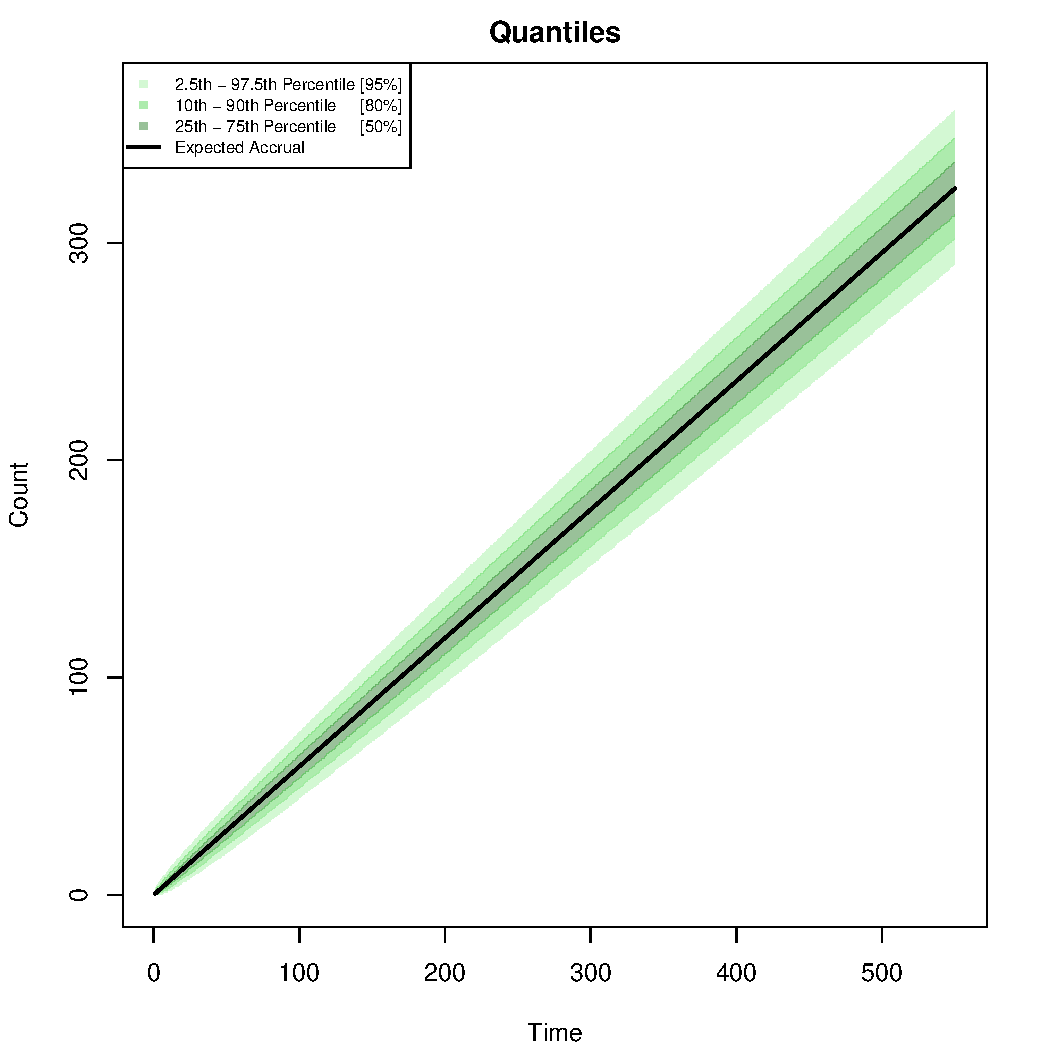
\includegraphics[width=\textwidth-3cm]{figure/ch02_figunnamed-chunk-6-1} 

}


\end{knitrout}
  \caption{Predicted uncertainty bands for Poisson process with $\lambda = 0.591$ over time. The black line represents the expected accrual, while the green shaded regions indicate aleatory uncertainty: the dark green band spans the interquantile range (25th - 75th percentiles), the lighter green band cover the 10th - 90th percentile range and the light green the 2.5th - 97.5th percentile range \citep{spiegelhalter2011visualizing}.}
  \label{fig:2_5}
\end{figure}
\newpage
\section{Counts: Negative Binomial model derived from Poisson-Gamma model}

The Negative Binomial $X\sim\rm{NBin}(r,\pi)$ models the number of 
\textit{trials} in a sequence of independent and identically distributed Bernouillis before $r$ \textit{successes} occur. Instead of representing the number of successes in $n$ trials like a $Y\sim \rm{Bin} (n, \pi)$, with the Negative Binomial we are looking at how many trials will it take to obtain $r$ successes.

With respect to the parameters, $r>0$ represents the number of successes until 
the experiment is stopped. The success probability in each experiment is 
represented by $\pi\in[0,1]$.  In R the functions \texttt{nbinom(..., size = r, prob = $\pi$)} relate to the random variable $X-r$, the number of successes (as opposed to the number of trials) until $r$ successes have been achieved \citep{held2014applied}. 

\begin{align*}
EX & = \frac{r(1-\pi)}{\pi}\\
Var(X) & = \frac{r(1-\pi)}{\pi^2}
\end{align*}


\subsection{Recruitment in one unit of time}
Let $Y|\Lambda \sim \rm{Po}(\Lambda)$ and $\Lambda \sim \rm{G}(\alpha,\beta)$
\begin{align*}
p(y)&=\int^\infty_0 p(y|\Lambda) p(\Lambda) d\Lambda\\
&=\int^\infty_0 \frac{\Lambda^y\exp(-\Lambda)}{y!}\Bigg[\Lambda^{\alpha-1}\exp(-\beta\Lambda)\frac{\beta^\alpha}{\Gamma(\alpha)}\Bigg]d\Lambda\\
&=\frac{\beta^\alpha}{y!\Gamma(\alpha)}\int^\infty_0 \Lambda^{\alpha+y-1}\exp(-\Lambda)\exp(-\Lambda\beta)d\Lambda\\
&=\frac{\Gamma(\alpha+y)}{y!\Gamma(\alpha)}\int^\infty_0 \beta^\alpha \exp(-\Lambda\beta)d\Lambda\\
&=\frac{\Gamma(\alpha+y)}{y!\Gamma(\alpha)}\Bigg(1-\frac{\beta}{\beta+1}\Bigg)^{\alpha}\Bigg(\frac{\beta}{\beta+1}\Bigg)^y \sim \rm{NBin} \Bigg(\alpha, \frac{\beta}{\beta+1}\Bigg)
\end{align*}
\newpage

Using the expressions of iterated expectation and variance \citep{held2014applied} and the expectation and variance from the respective random variables $Y|\Lambda \sim \rm{Po}(\Lambda)$ and $\Lambda \sim \rm{G}(\alpha,\beta)$, we have that:

\begin{align*}
EY &= E_{\Lambda}[E_{Y} (Y|\Lambda)] = E_{\Lambda}[\Lambda] = \alpha/\beta \\
Var(Y) &= Var_{\Lambda}[E_{Y} (Y|\Lambda)] + E_{\Lambda}[Var_Y(Y|\Lambda)]\\
&=Var_{\Lambda}[\Lambda] + E_{\Lambda}[\Lambda] \\
&=\alpha/\beta^2 + \alpha/\beta = \frac{\alpha(\beta+1)}{\beta^2}
\end{align*}

% 
% \begin{align*}
% Mean &= \frac{\alpha\bigg(1-\frac{\beta}{\beta+1}\bigg)}{\frac{\beta}{\beta+1}}\\
% &= \frac{\alpha\bigg (\frac{1}{\beta+1}\bigg)}{\frac{\beta}{\beta+1}}\\
% &= \frac{\alpha(\beta+1)}{\beta(\beta+1)}\\
% &= \frac{\alpha}{\beta}
% \end{align*}
% 
% \begin{align*}
% Variance &= \frac{\alpha\bigg(1-\frac{\beta}{\beta+1}\bigg)}{\bigg(\frac{\beta}{\beta+1}\bigg)^2}\\
% &= \frac{\alpha\bigg (\frac{1}{\beta+1}\bigg)}{\bigg(\frac{\beta}{\beta+1}\bigg)^2}\\
% &= \frac{\alpha(\beta+1)^2}{\beta^2(\beta+1)}\\
% &= \frac{\alpha(\beta+1)}{\beta^2}
% \end{align*}


\subsection{Accrual at time point t}
Let $Y|\Lambda \sim \rm{Po}(\Lambda t)$ and $\Lambda \sim \rm{G}(\alpha,\beta)$









